
% Distribución actual del corpus:
% Quepy questions 115
%   Recognized 58
%   Unrecognized 57
% Other questions 6658
%   Labeled 607
%   Unlabeled 6051

\chapter{Entorno de experimentación}

\section{Ejemplos seleccionados}\label{descripcion-corpus}

El primer paso antes de comenzar a experimentar fue conseguir las preguntas para construir un corpus. Son necesarios tanto ejemplos etiquetados que fueran la semilla de entrenamiento inicial de nuestro clasificador como un gran conjunto de ejemplos no etiquetados a partir de los cuales seleccionar instancias para enviar al oráculo.

Para el conjunto etiquetado comenzamos a partir de 58 ejemplos incluídos dentro de la aplicación de Quepy que describían posibles preguntas reconocidas por el programa. Es decir, estas 58 preguntas concuerdan con alguno de los patrones de la aplicación. Manualmente generamos reformulaciones para las cuales no existían patrones, aumentando el número de instancias etiquetadas a 115.

A partir de este punto comenzamos a buscar preguntas no etiquetadas. Utilizamos los corpus de entrenamiento y evaluación de los concursos del \textit{Text REtrieval Conference} (TREC) desde el año 1999 hasta el año 2007 \footnote{http://trec.nist.gov/data/qamain.html}. Esta competencia incluye preguntas de variados dominios y por ello la consideramos suficientemente representativa. Agregamos también las preguntas compiladas por \citet{corpus-stanford}, aunque no utilizamos la información adicional de este corpus. Obtuvimos un total de 6658 preguntas no etiquetadas.

Como último paso, etiquetamos otras 597 preguntas de este último conjunto que seleccionamos al azar. Aquí se introducen ejemplos etiquetados de preguntas que no pertenecen a ninguna clase semántica que pueda ser respondida por Quepy, y por lo tanto les asignamos la clase \textit{other}.

A partir de este conjunto de preguntas etiquetado separamos un porcentaje para evaluar el desempeño del clasificador de tal forma de que todas las clases estuvieran representadas en él. La distribución final de instancias se explica en la tabla \ref{dist-corpus}.

\begin{table}[h!]\label{dist-corpus}
\centering
\begin{tabular}{c c}
     & Cantidad de Instancias\\ [0.5ex]
    \hline
    Etiquetadas & 526 \\ [0.5ex]
    No etiquetadas & 6061 \\ [0.5ex]
    Para evaluación & 186 \\[1ex]
    \hline
\end{tabular}
\caption{Distribución de instancias.}
\end{table}

Sin embargo, algunos de los experimentos a realizar simularían las respuestas de un usuario a partir de etiquetas verdaderas. Dividimos entonces las instancias etiquetadas entre un corpus de entrenamiento y uno no etiquetado a partir del cual generar las respuestas simuladas. Para el corpus de entrenamiento seleccionamos una instancia de cada clase. El la tabla \ref{corpus-para-simulacion} se describe la configuración de estos corpus para simulaciones y en al apéndice \ref{ap-1} se incluye una tabla con la distribución de cada corpus por clase.

% Testing corpus: 31 recognized instances
% Testing corpus: 186 total instances
% Numbers of classes in Testing corpus  29
% Training corpus 19 recognized questions
% Training corpus total instances  29
% Unlabeled corpus 8 recognized instances
% Unlabeled corpus total instances  497

\begin{table}[h!]\label{corpus-para-simulacion}
\centering
\begin{tabular}{c c}
     & Cantidad de Instancias\\ [0.5ex]
    \hline
    Corpus de entrenamiento & 29 \\ [0.5ex]
    Corpus no etiquetado & 497 \\ [0.5ex]
    Corpus de evaluación & 186 \\[1ex]
    \hline
\end{tabular}
\caption{Distribución de instancias en los corpus para simulaciones}
\end{table}

\section{Preproceso}

Para poder comparar las preguntas con los patrones definidos en Quepy utilizamos el módulo de preproceso incluído en el mismo. Para la lematización y la extracción de etiquetas POS Quepy utiliza la librería \textit{nltk} desarrollada por \citet{nltk}, y a partir de esta información construye automáticamente objetos que pueden ser comparados con un patrón. El siguiente paso es comparar cada una de las preguntas procesadas con los patrones parciales de Quepy que extraemos de la misma aplicación. Adicionalmente utilizamos lemas y etiquetas POS para construir los bigramas, trigramas y bigramas mezclados.

Para obtener las entidades nombradas en las preguntas primero descargamos directamente desde FreeBase los nombres de posibles entidades. Debido a que la cantidad de infomación disponible es muy grande, restringimos nuestra búsqueda a entidades que probablemente estuvieran involucrados en preguntas de nuestro corpus. FreeBase organiza sus nodos asignándoles a cada uno varios tipos y decidimos tomar ventaja de esta característica para la selección de entidades.

Guiándonos por las clases de preguntas presenten en el corpus decidimos que los siguientes tipos eran relevantes: film\_actor, film\_director, books, book\_author, celebrities, locations, movies, musical\_group, musical\_group\_member, tv\_actor y tv\_show. Descargamos los nombres de todas las entidades de esos tipos y todos los otros tipos que tuvieran esas entidades.

Una vez obtenida esa información, comparamos cada nombre con cada pregunta para identificar si estaba contenido en ella o no. Si lo estaba, agregamos el nombre y sus tipos a la representación de la pregunta.

Al momento de procesar los corpus con las caraterísticas que ya mencionamos encontramos varios problemas. Una aproximación simple al aprendizaje activo incluye reentrenar el clasificador en cada una de las iteraciones del ciclo, cambiando así el modelo. Al introducir el etiquetado de características ya no se puede cambiar el modelo sin perder rastro de la ubicación de las características etiquetadas dentro de las matrices internas del clasificador. Por esto es que tuvimos que cambiar la implementación básica y extraer todos las características dentro del preproceso. De esta forma, nuestras matrices iniciales tienen todas las características tanto del corpus anotado como no anotado, aunque en cada corpus por separado muchas columnas contengan sólo ceros.



\section{Métricas utilizadas}
\begin{description}
    \item[\textit{Accuracy}] Llamamos \textit{Accuracy} a la cantidad de preguntas etiquetadas correctamente sobre el total de preguntas clasificadas. Utilizamos el nombre en inglés debido a la falta de una traducción adecuada y para evitar confusiones con la métrica Precisión que describiremos a continuación.
    \item[Curva de aprendizaje] Definimos la curva de aprendizaje como la \textit{accuracy} en función de la cantidad de ejemplos o características etiquetados utilizados para entrenar al clasificador.
    \item [Coeficiente Kappa de Cohen] Esta medida ajusta el \textit{accuracy} del clasificador utilizado a la de un clasificador aleatorio o tonto. Un \textit{accuracy} del 80\% no es muy sorprendente si asignando etiquetas al azar obtenemos un \textit{accuracy} del 70\%. En nuestro caso el corpus de evaluación contiene aproximadamente un 75\% de instancias de clase ``otro'', por lo tanto un clasificador que elija esta etiqueta todas las veces obtendría un \textit{accuracy} semejante. Esta métrica nos permitirá medir más adecuadamente el desempeño del clasificador.\\
    Una definición más formal del Coeficiente de Kappa es la que propone \citet{KappaCarletta}:
    $$K = \frac{P(A)-P(E)}{1-P(E)}$$
    donde $P(A)$ es la proporción de veces que los clasificadores acuerdan y $P(E)$ es la proporción de veces que se esperaría que acuerden por casualidad. En este caso, uno de los clasificadores es el Multinomial bayesiano entrenado y el otro son las etiquetas del corpus de evaluación. Por lo tanto, $P(A)$ no es otra cosa más que la \textit{accuracy} calculada en el primer item. Adicionalmente, calculamos $P(E)$ de la siguiente forma:
    $$P(E) = \frac{\sum_{i\in\mathcal{C}}Pr(\hat{x_i})*Pr(x_i)}{|\mathcal{E}|}$$
    donde $\mathcal{C}$ es el conjunto de clases, $\mathcal{E}$ es el corpus de evaluación, $Pr(\hat{x_i})$ es la proporción de instancias etiquetadas por el clasificador con la clase i, y $Pr(x_i)$ es la proporción de instancias que pertenecen realmente a la clase i.
    % http://stats.stackexchange.com/questions/82162/kappa-statistic-in-plain-english
    \item [Precisión y exhaustividad por clase] Estas dos medidas puede utilizarse sólo en clasificación binaria, por lo que tomaremos sus valores para cada una de las clases posibles. Definimos precisión como la cantidad de instancias etiquetadas para una clase que son correctas (positivos verdaderos o $P_v$) sobre la cantidad de instancias etiquetadas para esa clase ($P_v$ y falsos positivos o $P_f$).
    $$Precision(C_i) = \frac{P_v}{P_v + P_f}$$
    La exhaustividad, por otro lado, está definida como la cantidad de instancias etiquetadas correctamente ($P_v$) de una clase dada sobre la cantidad de instancias que pertenecen a la clase verdaderamente ($P_v$ y falsos negativos o $N_f$).
    $$Exhaustividad(C_i) = \frac{P_v}{P_v + N_f}$$
    \item[Reconocimiento] Definimos esta métrica como \textit{Accuracy} pero calculada sólo sobre la porción del corpus de evaluación que no es de la clase ``otro''. Con esto podremos medir si el clasificador está ampliando la cobertura de las clases semánticas, sin ser abrumados por la gran cantidad de preguntas de la clase mayoritaria en el corpus de evaluación. Tengamos en cuenta que la pérdida acarreada por no identificar una pregunta que puede ser respondida por Quepy es mucho mayor que clasificar una pregunta con una clase semántica que no le corresponde. En el segundo escenario, el sistema simplemente construirá una consulta y la enviará al motor de búsqueda, obteniendo en la mayoría de los casos una respuesta vacía. Por ello es que tomaremos el reconocimiento como una medida más significativa que el \textit{accuracy}.
    \item[Curva de reconocimiento] Análogamente a la curva de aprendizaje, definimos la curva de reconocimiento como el reconocimiento del clasificador en función de la cantidad de ejemplos o características etiquetados utilizados para entrenarlo.
\end{description}

\chapter{Experimentos}

En este capítulo explicaremos cada uno de los experimentos que realizamos. Las hipótesis a validar abarcan desde la representación elegida y preproceso hasta la utilidad del aprendizaje activo. Por ello, describimos los experimentos en el orden en que los fuimos desarrollando, ya que los resultados de cada uno de ellos cambiaron las hipótesis iniciales de los restantes e incluso generaron nuevos experimentos.

Todos los gráficos de esta sección son generados a partir de los datos con un suavizamiento para que sean más fáciles de interpretar.

\section{Experimento 1}
\vspace{3 mm}
\textbf{Hipótesis} El clasificador \textit{MultinomialNB} básico de la librería \textit{scikit-learn} obtiene buenos resultados utilizando aprendizaje supervisado y entrenando con el corpus etiquetado.
\vspace{3 mm}

Este es el primer experimento que realizamos para obtener una base de desempeño con la cual medir luego nuestro clasificador. Utilizamos el corpus completo de entrenamiento y obtenemos las métricas a partir del corpus de evaluación tal y como fueron descriptos en la sección \ref{descripcion-corpus}.
Adicionalmente, realizamos el mismo proceso con otros clasificadores populares en clasificación de texto: \textit{Support Vector Machine} (SVM) desarrollado por \citet{svm-cortes} y \textit{Decision Trees}, mencionados ambos en \citet{Sebastiani-text-categorization}.

Los dos nuevos clasificadores utilizados pertenecen también a la librería \textit{scikit-learn} de \citet{scikit-learn}. Son instancias de las clases \textit{sklearn.tree.DecisionTreeClassifier} y \textit{sklearn.svm.SCV} respectivamente que dejamos con sus parámetros predeterminados por defecto. \citet{svm-uso-Joachims} ha obtenido buenos resultados usando SVM y sostiene que elimina la necesidad de utilizar selección de características. Por estos dos motivos consideramos la comparación adecuada.

Incluimos estos clasificadores dentro de un ciclo de aprendizaje activo sólo sobre instancias simulado para analizar el posible beneficio de este método. En todos los casos las instancias fueron seleccionadas eligiendo primero las de mayor entropía. Destacamos que aunque el aprendizaje activo es sólo sobre instancias, estamos utilizando el módulo \textit{ActivePipeline} y llevando a cabo un paso del algoritmo Esperanza-Maximización para el clasificador \textit{MultinomialNB}.

\vspace{3 mm}

\textbf{Resultados} En la siguiente tabla se muestran el \textit{accuracy}, el reconocimiento y el coeficiente kappa para los tres clasificadores \textit{MultinomialNB} (MNB), \textit{Support Vector Machine} (SVM) y \textit{Decision Trees} (DT).

\begin{table}[h]
\centering
\begin{tabular}{l c c c}
     & MNB & SVM & DT\\ [0.5ex]
    \hline
    \textit{Accuracy} & 0.725 & 0.725 & 0.655 \\ [0.5ex]
    Coeficiente kappa & 0.000 & 0.000 & 0.235 \\ [0.5ex]
    Reconocimiento & 0.000 & 0.000 & 0.235 \\[1ex]
    \hline
\end{tabular}
\caption{Comparación de rendimiento sobre el corpus de evaluación}
\end{table}

% python experiments/grapich_learning_curves.py experiments/results/experiment4/learningcurve-full-186-step2-unbalance "Curva de aprendizaje" experiments/results/experiment4/recognitioncurve-full-186-step2-unbalance "Curva de reconocimiento"
\begin{figure}[h!]\label{curva-apr-vs-rec-dt}
\centering
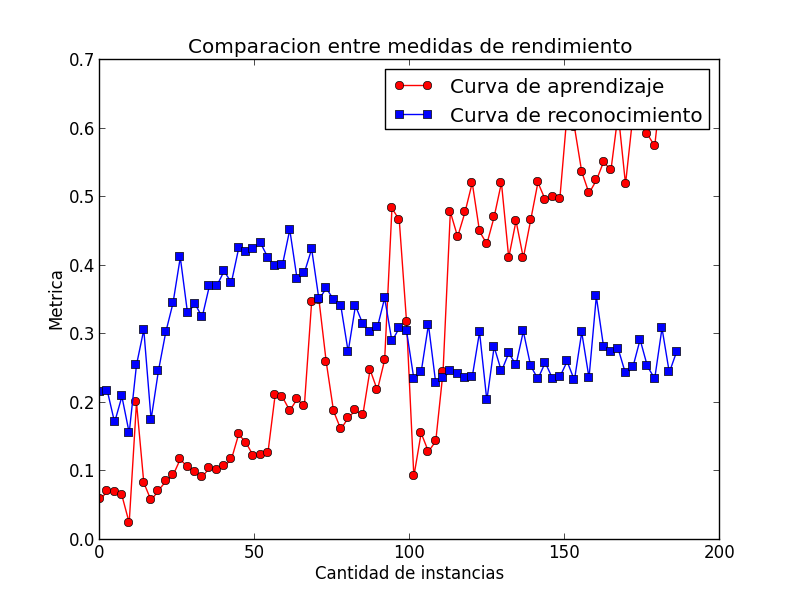
\includegraphics[width=12cm]{curva-apr-vs-rec-dt}
\caption{Curvas de aprendizaje y reconocimiento para el clasificador DT comenzando con un corpus de 29 instancias etiquetadas.}
\end{figure}

El valor las tres medidas en los clasificadores SVM y MNB durante el aprendizaje activo se mantiene constante luego de superar las 10 instancias agregadas al corpus de entrenamiento.

\vspace{3 mm}

\textbf{Conclusión}
Si observáramos aisladamente la medida del \textit{accuracy} para este experimento podría pensarse que todos los clasificadores obtienen resultados significativos, o al menos aceptables. Sin embargo el reconocimiento y el factor kappa ponen en relevancia que los clasificadores MNB y SVM sólo reconocen la clase mayoritaria y etiquetan con ella a todas las instancias.

La figura \ref{curva-apr-vs-rec-dt} con el desempeño en el aprendizaje activo del clasificador DT da indicios de porqué sucede este fenómeno. Si bien el \textit{accuracy} logrado es más bajo, el reconocimiento es más alto en el clasificador final. Analizando las dos curvas de aprendizaje podemos ver que el reconocimiento alcanza su punto máximo con un valor de 0.45 con 60 instancias agregadas al corpus de entrenamiento y posteriormente decae hasta su valor final. Como las primeras instancias agregadas son las de mayor entropía, corresponden a instancias que no pertenecen a la clase mayoritaria. Por lo tanto, formulamos la hipótesis de nuestro experimento número 2 de que entrenar el clasificador con pocas instancias de la clase mayoritaria aumentaría el reconocimiento final.

\section{Experimento 2}
\vspace{3 mm}
\textbf{Hipótesis} Entrenar el clasificador \textit{MultinomialNB} básico de la librería \textit{scikit-learn} con un corpus de entrenamiento con una cantidad reducida de instancias de clase mayoritaria aumenta el reconocimiento, mientras reduce el \textit{accuracy}.
\vspace{3 mm}

Para realizar este experimento medimos cómo se comporta el \textit{accuracy} y el reconocimiento en función de la cantidad de instancias de clase mayoritaria con que se entrena al clasificador. Es decir, comenzamos con un clasificador entrenado con todas las instancias etiquetadas de clases minoritarias de las que disponemos, 129 en total. Luego agregamos paulatinamente instancias de clase mayoritaria y reentrenamos el clasificador.

Para tener una línea de comparación, también realizamos el mismo proceso con los dos clasificadores utilizados en el experimento anterior.

\vspace{3 mm}

\textbf{Resultados} En las siguientes imágenes se muestran los valores del \textit{accuracy} y el reconocimiento para los tres clasificadores \textit{MultinomialNB} (MNB), \textit{Support Vector Machine} (SVM) y \textit{Decision Trees} (DT), utilizando una estrategia de selección de instancias priorizando máxima entropía.

\begin{figure}[h!]\label{curva-apr-hip2}
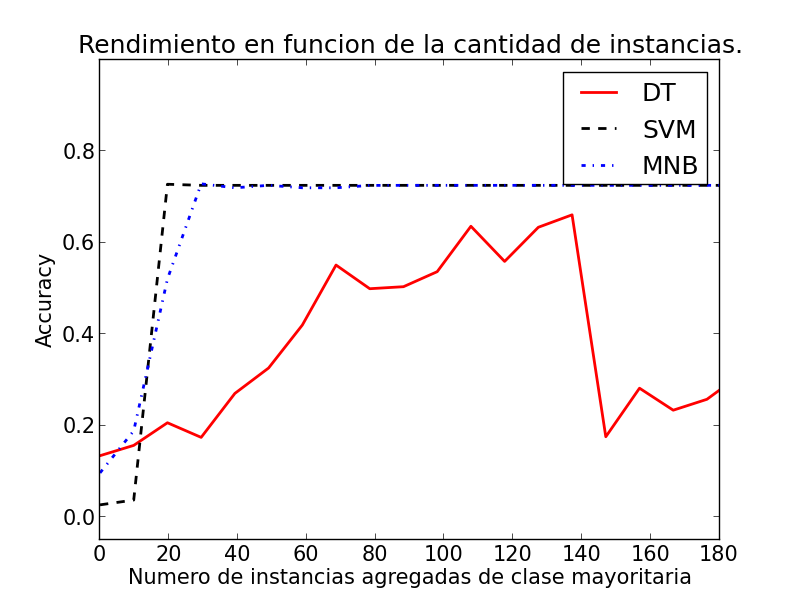
\includegraphics[width=8cm]{learning-curve-hip2}
%python experiments/grapich_learning_curves.py experiments/results/experiment4/learningcurve-full-186-step2-hip2 "DT" experiments/results/experiment5/learningcurve-full-186-step2-hip2 "SVM" experiments/results/experiment2/learningcurve-full-186-step1-hip2 "MNB"
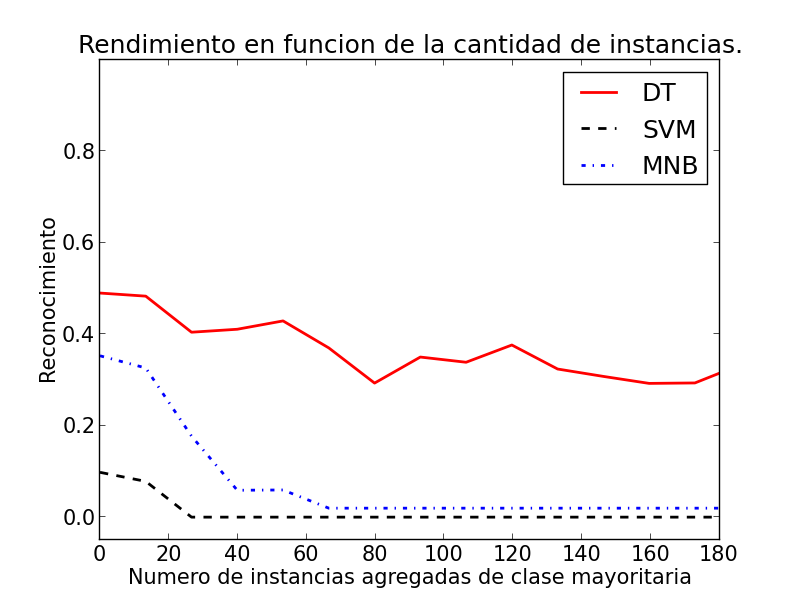
\includegraphics[width=8cm]{recognition-curve-hip2}
% python experiments/grapich_learning_curves.py experiments/results/experiment4/recognitioncurve-full-186-step2-hip2 "DT" experiments/results/experiment5/recognitioncurve-full-186-step2-hip2 "SVM" experiments/results/experiment2/recognitioncurve-full-186-step1-hip2 "MNB"
\caption{Curvas de aprendizaje y reconocimiento en función de la cantidad de instancias de la clase mayoritaria utilizadas en el entrenamiento para los clasificadores DT, SVM y MNB.}
\centering
\end{figure}

\vspace{3 mm}

\textbf{Conclusión}
Como esperábamos, el reconocimiento es inversamente proporcional a la cantidad de instancias de clase mayoritaria que se utilizan en el entrenamiento. Esto no quiere decir que no deban ser utilizadas, sino que pueden estar abrumando los pocos datos etiquetados de las otras clases que componen el corpus de entrenamiento.

Estos resultados no son extraños en problemas donde se busca reconocer y clasificar una pequeña parte del universo de instancias, como ya hemos visto que plantea \citet{rare-classes-holpedales}. En nuestro caso, estamos clasificando el resto del universo dentro de una clase mayoritaria aunque esto no se corresponda con la realidad. Esta mega-clase engloba las instancias de todas las clases que no podemos reconocer, y como tal no existen características distintivas que permitan al clasificador reconocerlas. Ante tanta diversidad, como podemos observar el desempeño es pobre y se basa sólo en la probabilidad mayor de una etiqueta.


\section{Nueva configuración del corpus}

Como resultado del experimento anterior utilizaremos a partir de ahora un corpus no etiquetado (simulado) con la misma cantidad de instancias de la clase mayoritaria que de la segunda clase mayoritaria, es decir, 14 instancias. Si bien esto constituye un corpus muy pequeño, queremos identificar tendencias y no resultados contundentes dado los limitados recursos de los que disponemos.

Al realizar las primeras pruebas tentativas para este corpus notamos que la precisión no podía ser calculada para aquellas clases que se entrenaban con menos de 4 instancias. Esto se debe a que el clasificador no clasifica ninguna instancia como perteneciente a esta clase, lo que resulta en una división por 0 al calcular la métrica. Tengamos en cuenta de que son sólo 4 las instancias que podemos incluir en el corpus de entrenamiento porque previamente seleccionamos 1 o 2 para el corpus de evaluación.

La base de la clasificación es la generalización de la información de los datos de entrenamiento a instancias nunca vistas previamente. La poca cantidad de reformulaciones que pudimos encontrar para estas preguntas conduce a la conclusión de que estas clases no podrán ser discriminadas sin incluir más ejemplos. Por ello tomamos la decisión de excluir estas clases de los siguientes experimentos considerando que no aportan ningún beneficio ni perjuicio a los datos que queremos observar. Se eliminan en este paso 17 clases que representan un 37\% del corpus de entrenamiento y no etiquetado, mientras que sólo es un 10\% del corpus de evaluación. Las clases seleccionadas y la estructura final de los corpus para simulaciones se detalla en el apéndice \ref{ap-2}.


\section{Experimento 3}
\vspace{3 mm}
\textbf{Hipótesis} Las características como las concordancias parciales y los tipos de entidades nombradas son más significativas que las otras para el clasificador \textit{MultinomialNB}.
\vspace{3 mm}

Antes de comenzar con el entrenamiento a través de aprendizaje activo propiamente dicho queremos determinar la configuración de experimentos que maximizará el resultado final. Como mencionamos en el capítulo \ref{capitulo-features}, consideramos que este grupo de características representa mejor a las instancias para esta tarea de categorización en particular. Las preguntas que queremos analizar tienen una longitud corta y un vocabulario similar, es decir, muchas preguntas contiene palabras como \textit{What}, \textit{Who} o \textit{is}. Sin embargo, estas palabras no son discriminatorias de la clase en la mayoría de los casos, sino que dependemos del resto de la frase. Por otro lado, al tener una alta cantidad de clases distintas, es probable que cada una de estas palabras discriminatorias esté presente en pocos ejemplos, si no sólo en uno, resultando en un matriz de representación muy dispersa. Por estos motivos suponemos que utilizar derivados simples de las lemas no formará una frontera de decisión tan clara para el clasificador.

Para probar esta hipótesis entrenamos el clasificador \textit{MultinomialNB} con el corpus de entrenamiento y no etiquetado (simulado) descriptos en la sección anterior preprocesados con distintas combinaciones de características. Para un mejor entendimiento de los datos, realizamos un análisis sobre el corpus usado para entrenamiento y obtenemos la distribución de ocurrencias de cada tipo de características en las instancias.

\vspace{3 mm}

\textbf{Resultados} En la siguiente tabla mostramos las mediciones más significativas de \textit{accuracy} y reconocimiento obtenidas sin aprendizaje activo para combinaciones de los siguientes tipos de características: Lemas (L), Bigramas (B), Trigramas (T), Bigramas Mezclados (MB), Etiquetas POS (POS), Entidades nombradas (NE), Tipos de las entidades nombradas (NET) y Concordancia a patrones parciales (PM).

\begin{table}[h!]\label{tabla-exp3}
\centering
\begin{tabular}{l c c}
     & \textit{Accuracy} & Reconocimiento \\ [0.5ex]
    \hline
    Todos & 0.31 & 0.46 \\[0.5ex]
    L & 0.49 & 0.59 \\ [0.5ex]
    L + B & 0.40 & 0.59 \\ [0.5ex]
    \textbf{L + B + T} & 0.32 & \textbf{0.71} \\[0.5ex]
    L + B + T + MB + POS & 0.30 & 0.59 \\[0.5ex]
    L + B + T + NET + NE & 0.35 & 0.59 \\[0.5ex]
    L + B + T + PM & 0.40 & 0.59 \\[0.5ex]
    L + B + T + PM + NET & 0.39 & 0.53 \\[0.5ex]
    L + PM & 0.43 & 0.59 \\[0.5ex]
    L + PM + NET & 0.50 & 0.46 \\[0.5ex]
    L + PM + NET + NE & 0.52 & 0.46 \\[0.5ex]
    \textbf{PM} & 0.40 & \textbf{0.65} \\[0.5ex]
    PM + NET & 0.60 & 0.53 \\[0.5ex]
    \textbf{PM + NET + NE} & \textbf{0.64} & 0.43 \\[0.5ex]
    \hline
\end{tabular}
\caption{Comparación de desempeño sobre el corpus de evaluación}
\end{table}

En la figura \ref{fig-distribucion-features} cada gráfico de torta ilustra la cantidad de características que ocurren en un número fijo de instancias distribuidas según la clase a la que pertenecen. Es decir, en el primer gráfico la porción de color negro representa cuántos lemas (L) aparecen sólo en una pregunta de todo el corpus.

\begin{figure}[h!]\label{fig-distribucion-features}
\centering
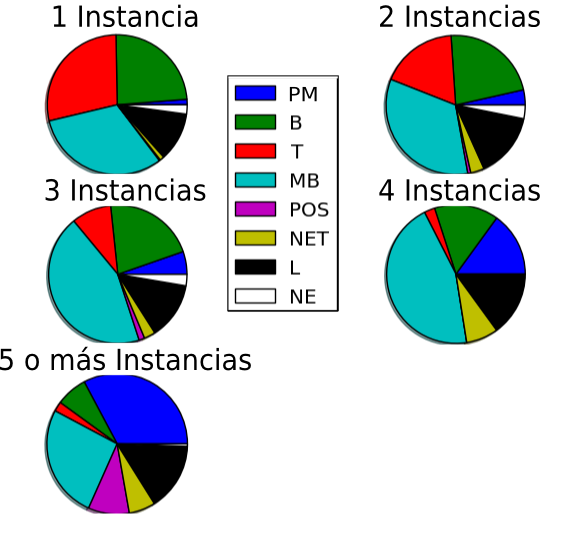
\includegraphics[width=10cm]{clase-feat-inst-labels}
\caption{Distribución de las clases de las características según la cantidad de instancias en las que están presentes.}
\end{figure}

\vspace{3 mm}

\textbf{Conclusión} Primero realizaremos un análisis de los gráficos de torta y luego ahondaremos en el desempeño del clasificador a partir de esa base. Lo primero que notamos es que, como habíamos supuesto, la proporción de Concordancias parciales (PM) y Tipos de entidades nombradas (NET) aumenta mientras aumenta el número de instancias en las que están presentes. Es decir, en proporción hay muchas más reglas que concuerdan con muchas instancias que con una sola. Lo mismo ocurre con las etiquetas POS, pero recordemos que hay pocas de ellas y que en general ocurren muchas veces en el texto. Es decir, en todas las frases hay sustantivos y verbos. Por lo tanto, no las consideraremos relevantes. Sin embargo, sí encontramos significativo que la proporción de los lemas se mantenga constante con respecto a la cantidad de instancias en las que ocurren. Esto nos indica que esta característica podría ser mucho más útil de lo que esperábamos.

El fenómeno contrario ocurre con los Bigramas (B) y Trigramas (T), junto con las Entidades Nombradas en sí (NE), que en general ocurren en pocas instancias dentro del corpus. Por lo tanto, esperaríamos que no se desempeñen bien aisladas sino en conjunto con otras características.

Con respecto al rendimiento del clasificador, ninguna combinación de características maximiza tanto el \textit{accuracy} como el reconocimiento. Es decir, que para identificar mejor las instancias de las clases minoritarias es necesario perder precisión sobre la clase mayoritaria. Recordemos que para el fin de nuestra clasificación preferimos lograr un alto reconocimiento.

A partir de la tabla \ref{tabla-exp3} podemos observar claramente que el mayor reconocimiento se obtiene utilizando Concordancias a los patrones (PM) o la combinación Lemas, Bigramas y Trigramas. Sin embargo, la combinación de estos no arroja buenos resultados. Una causa posible para esto puede ser que parte de la información aportada por los Lemas, Bigramas y Trigramas es opacada por la fuerte presencia de las Concordancias a patrones y viceversa. ALGO MAS TENGO QUE PONER!

Por otra parte, los Tipos de las entidades nombradas y las Entidades nombradas sólo aumentan el \textit{accuracy} pero reducen el reconocimiento. Si observamos la figura \ref{fig-distribucion-features} estos tipos de características son muy dispersas y ocurren generalmente en menos de tres instancias. Además de ello, muchas de las preguntas de clase \textit{other} no tienen entidad nombrada, por lo tanto son una característica que permite separar mejor el universo entre la clase mayoritaria y las demás.

\section{Experimento 4}
\vspace{3 mm}
\textbf{Hipótesis} La clasificación obtendrá mejores resultados si se aplica algún método de suavizado como \textit{Tf-idf} o \textit{LSA}.
\vspace{3 mm}

Métodos de suavizado son utilizados comúnmente en la clasificación de texto y extracción de información para contrarrestar la distribución de palabras descripta por la ley de Zipff, donde pocas palabras ocurren muchas veces mientras que la mayoría de los términos están presentes en pocas instancias.

\textit{Tf-Idf} hace referencia a Frecuencia de términos y frecuencia inversa de documentos, una medida estadística para determinar cuán importante es una palabra dentro de una instancia o documento. Se calcula como el producto de otras dos medidas: la Frecuencia del término es la cantidad de veces que una característica ocurre en la instancia, y la Frecuencia inversa del documento es la inversa de la cantidad de veces que la característica aparece en todo el corpus. Como resultado, palabras que ocurren pocas veces en el corpus y se concentran sólo en una porción de instancias toman más relevancia con respecto a palabras que ocurren en muchas instancias, ya que se consideran más representativas. Ha sido utilizado por \citet{tackling-mnb} como una forma de modelado alternativa para el clasificador Bayesiano ingenuo.

\textit{LSA} o Análisis de semántica latente es una técnica introducida por \citet{lsa} para superar los problemas de utilizar aproximaciones basadas sólo en términos para el procesamiento de lenguaje natural. Supone que existe una estructura semántica oculta por la aleatoriedad del vocabulario e intenta minimizar el ruido a través de técnicas estadísticas. \textit{LSA} utiliza una técnica llamada Descomposición en valores singulares o \textit{SVD} que descompone la matriz de representación en un nuevo espacio vectorial de forma que se reduce la dimensionalidad (tiene menos características) mientras se preserva la relación entre las las características restantes y las instancias.

Para aplicar estos dos métodos usamos las clases \textit{TfidfTransformer} y \textit{TruncatedSVD} de la librería \textit{scikit-learn}. Luego de preprocesar todos los corpus con estos métodos entrenamos el clasificador \textit{MultinomialNB} y comprobamos su rendimiento sobre el corpus de evaluación.

\vspace{3 mm}

\textbf{Resultados} En la siguiente tabla mostramos las mediciones más significativas de \textit{accuracy} y reconocimiento obtenidas sin aprendizaje activo para combinaciones de las siguientes características: Lemas (L), Bigramas (B), Trigramas (T), Bigramas Mezclados (MB), Etiquetas POS (POS), Entidades nombradas (NE), Tipos de las entidades nombradas (NET) y Concordancia a patrones parciales (PM), aplicando métodos de suavizado de Tf-idf y LSA. Entre paréntesis se incluye la diferencia de cada métrica con respecto a los resultados de la tabla \ref{tabla-exp3}.

\begin{table}[h]\label{tabla-exp4}
\centering
\begin{tabular}{l c c | c c}
     & \multicolumn{2}{c|}{Tf-Idf} & \multicolumn{2}{c}{LSA}\\ [0.5ex]
     & \textit{Accuracy} & Reconocimiento & \textit{Accuracy} & Reconocimiento \\ [0.5ex]
    \hline
    Todos & 0.32(+.01) & 0.40($-$.06) & 0.67(+.36) & 0.53(+.07) \\[0.5ex]
    L & 0.45($-$.04) & 0.40($-$.19) & 0.72(+.30) & 0.37($-$.22) \\[0.5ex]
    L + B + T & 0.36(+.04) & 0.34($-$.37) & 0.74(+.42) & 0.43($-$.28) \\[0.5ex]
    PM & 0.44(+.04) & \textbf{0.59}($-$.06) & 0.41(+.01) & 0.43($-$.22) \\[0.5ex]
    \textbf{PM + L} & 0.35($-$.08) & 0.50($-$.09) & 0.44(+.01) & \textbf{0.68}(+.09) \\[0.5ex]
    PM + L + NET & 0.50(+.00) & 0.50(+.04) & \textbf{0.79}(+.29) & 0.25($-$.21)\\[0.5ex]
    \textbf{PM + L + B + T} & 0.32($-$.08) & 0.46($-$.13) & 0.49(+.09) & \textbf{0.68}(+.09) \\[0.5ex]
    PM + L + B + T + NET & 0.40(+.01) & 0.43($-$.10) & \textbf{0.79}(+.30) & 0.31($-$.22) \\[0.5ex]
    PM + NET + NE & \textbf{0.64}(+.00) & 0.43(+.00) & 0.74(+.10) & 0.09($-$.34) \\[0.5ex]
    PM + NET + NE + L & 0.52(+.00) & 0.46(+.00) & 0.76(+.24) & 0.21($-$.25) \\[0.5ex]
    \hline
%    Todos & 0.32 & 0.4 & 0.67 & 0.53 \\[0.5ex]
%    L & 0.45 & 0.4 & 0.72 & 0.37 \\[0.5ex]
%    L + B + T & 0.36 & 0.34 & 0.74 & 0.43 \\[0.5ex]
%    PM & 0.44 & \textbf{0.59} & 0.41 & 0.43 \\[0.5ex]
%    \textbf{PM + L} & 0.35 & 0.5 & 0.44 & \textbf{0.68} \\[0.5ex]
%    PM + L + LNT & 0.50 & 0.50 & 0.79 & 0.25\\[0.5ex]
%    \textbf{PM + L + B + T} & 0.32 & 0.46 & 0.49 & \textbf{0.68} \\[0.5ex]
%    PM + L + B + T + LNT & 0.40 & 0.43 & 0.79 & 0.31 \\[0.5ex]
%    PM + LTN + LN & \textbf{0.64} & 0.43 & 0.74 & 0.09 \\[0.5ex]
%    PM + LTN + LN + L & 0.52 & 0.46 & \textbf{0.76} & 0.21 \\[0.5ex]
\end{tabular}
\caption{Comparación de desempeño sobre el corpus de evaluación con distintas caraterísticas y técnicas de suavizamiento.}
\end{table}
% L + PM + NET + NE + B + T + MB + POS
No incluimos los resultados de los experimentos utilizando ambos métodos ya que ninguno de ellos dio mejores resultados que los mencionados anteriormente.

Los datos expresados con el preprocesamiento de LSA tienen el número de dimensiones que maximizan el resultado. Para las combinaciones más exitosas PM + L + B + T y PM + L se utilizaron 250 características.

En la tabla \ref{prec-recall-mejor-solucion} se muestra la precisión y la exhaustividad para cada una de las clases utilizando las dos mejores combinaciones de características de la tabla \ref{tabla-exp3}. En la última columna se incluye el número de instancias para cada clase dentro del corpus de evaluación.

\begin{table}[h]\label{prec-recall-mejor-solucion}
\centering
\begin{tabular}{l c c | c c | c}
     & \multicolumn{2}{c|}{PM + L + B + T + LSA} & \multicolumn{2}{c}{PM + L + LSA} &\\ [0.5ex]
    Clase & Precisión & Exhaustividad & Precisión & Exhaustividad & Instancias\\ [0.5ex]
    \hline
    actedon & 0.57 & 1.00 & 0.57 & 1.00 & 4\\ [0.5ex]
    \textbf{albumsofband} & 0.33 & 0.80 & \textbf{0.36} & \textbf{0.86} & 5\\ [0.5ex]
    bandmembers & 1.00 & 0.50 & 1.00 & 0.50 & 2\\ [0.5ex]
    \textbf{booksbyauthor} & \textbf{1.00} & 0.67 & 0.50 & 0.67 & 3\\ [0.5ex]
    castof & 0.00 & 0.00 & 0.00 & 0.00 & 1\\ [0.5ex]
    \textbf{creatorof} & \textbf{0.17} & 1.00 & 0.15 & 1.00 & 2\\ [0.5ex]
    \textbf{howoldis} & \textbf{0.09} & 1.00 & 0.08 & 1.00 & 5\\ [0.5ex]
    \textbf{other} & 0.92 & \textbf{0.44} & \textbf{0.93} & 0.38 & 135\\ [0.5ex]
    presidentsof & 0.50 & 0.50 & 0.50 & 0.50 & 2\\ [0.5ex]
    showswith & 0.00 & 0.00 & 0.00 & 0.00 & 1\\ [0.5ex]
    \textbf{whereis} & \textbf{0.38} & 1.00 & 0.33 & 1.00 & 3\\ [0.5ex]
    whereisfrom & 0.00 & 0.00 & 0.00 & 0.00 & 4\\ [0.5ex]
    & & & & & \\
    Promedio/total & \textbf{0.82} & \textbf{0.49} & 0.81 & 0.44 & 167\\ [0.5ex]
    \hline
\end{tabular}
\caption{Precisión y exhaustividad sobre el corpus de evaluación con dos combinaciones de características y LSA.}
\end{table}


\vspace{3 mm}

\textbf{Conclusión}
La técnica \textit{Tf-Ifd} mejora en un porcentaje muy bajo el \textit{accuracy} en algunos casos, mientras que para la mayoría de las combinaciones reduce el reconocimiento. Observamos que en general aplicar esta técnica reduce los valores en la matriz de representación. Por ejemplo, para la combinación de características L + B + T + PM + NET el valor máximo de dicha matriz es 0.43, mientras que su media es 0.0014 teniendo un 1.1\% de valores no nulos. Sin \textit{Tf-Ifd} la media de valores de la matriz de representación es 0.011 y el valor máximo 6. Como resultado, al clasificar la probabilidad de la clase tiene más importancia utilizando esta técnica y la mayoría de las etiquetas es alguna de las clases con más instancias.

Por otro lado, como esperábamos, agregar \textit{LSA} permite combinar mejor los Lemas, Bigramas y Trigramas con las Concordancias a patrones. Aún si esta combinación no alcanza los valores de reconocimiento que pudimos observar en el experimento anterior, aumenta significativamente el \textit{accuracy}. Vemos que este en un fenómeno general de todas las combinaciones, por lo que esperamos que con un corpus mayor esta técnica permita aumentar el rendimiento sobre todas las clases. Insistimos en agregar más características que Lemas, Bigramas y Trigramas ya que tenemos la intuición de que con mayor cantidad de ejemplos y un vocabulario más amplio éstas no serían suficientes.

Un resultado sorprendente es el bajo reconocimiento de la combinación L + B + T con LSA, que en el experimento anterior obtuvo los mejores resultados. Un fenómeno común que observamos al reducir la dimensionalidad es que la clase mayoritaria vuelve a adquirir un gran peso. Por ello aumenta tanto el \textit{accuracy} de todas las combinaciones.

La tabla \ref{prec-recall-mejor-solucion} indica, con un análisis más detallado, que la mejor combinación de características es L + B + T + PM + LSA. La adición de Bigramas y Trigramas mejora el \textit{accuracy} permitiendo ... POR QUÉ????

\section{Experimento 5}\label{experimento-aa-instancias}
\vspace{3 mm}
\textbf{Hipótesis} El aprendizaje activo sobre instancias permite al clasificador obtener el mismo rendimiento con menor cantidad de instancias.
\vspace{3 mm}

En este experimento simulamos la interacción con un usuario como describimos en la sección \ref{descripcion-corpus}, comenzando con un corpus de entrenamiento pequeño el ciclo de aprendizaje activo. El aprendedor selecciona la siguiente instancia de un corpus etiquetado (sin conocer la verdadera clase) para enviar al oráculo, pero en lugar de interactuar con un usuario obtenemos las respuestas del mismo corpus.

Para esta sección decidimos preprocesar los datos utilizando Lemas, Bigramas, Trigramas y Concordancias a patrones y aplicando LSA, basándonos en los resultados del experimento anterior. Evaluaremos la curva de aprendizaje y de reconocimiento con tres estrategias de selección de instancias distintas: al azar, con mayor entropía y con menor entropía. El clasificador utilizado es \textit{MultinomialNB} junto con el módulo ActivePipeline.

Recordemos que las instancias con menor entropía son aquellas sobre las que el clasificador tiene mayor seguridad, y por lo tanto aportan menos información. Seleccionar instancias con menor entropía primero permitirá al clasificador asegurar la información que se asume es verdadera. Consideramos que esta es una buena estrategia teniendo en cuenta la reducida cantidad de ejemplos con los que comienza el entrenamiento del clasificador.

El clasificador se reentrenó y se aplicó un ciclo del algoritmo Esperanza-Maximización luego de agregar una instancia al corpus de entrenamiento.

\vspace{3 mm}

\textbf{Resultados} En la figura \ref{fig-aa-comparision} mostramos la evolución del \textit{accuracy} y del reconocimiento para las tres estrategias de selección de instancias: aleatoria, mayor entropía y menor entropía. Para graficar las curvas utilizando selección aleatoria se promedian los valores obtenidos de cada métrica de 5 experimentos distintos.

\begin{figure}[h!]\label{fig-aa-comparision}
\centering
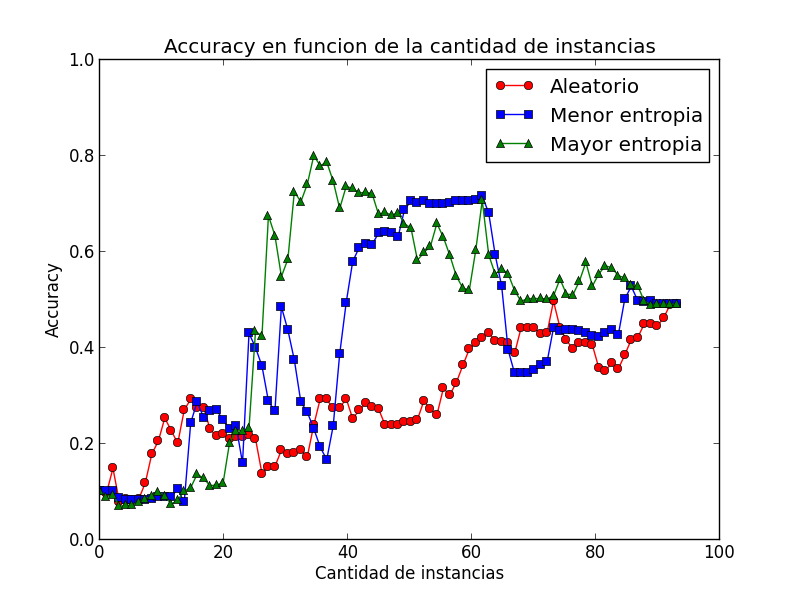
\includegraphics[width=10cm]{learningcurve-aa-exp5}
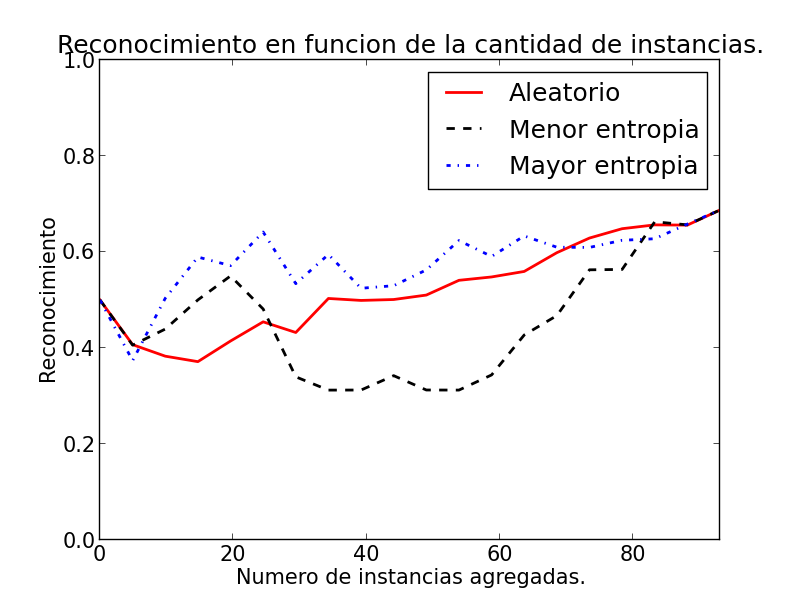
\includegraphics[width=10cm]{recognitioncurve-aa-exp5}
\caption{Desempeño del clasificador con aprendizaje activo y distintas estrategias de selección de instancias.}
\end{figure}

\vspace{3 mm}

\textbf{Conclusión}
Como podemos observar en la curva de aprendizaje ambas estrategias se desempeñan mejor que un aprendizaje aleatorio. Sin embargo, la selección por mayor entropía maximiza tanto el \textit{accuracy} como el reconocimiento.

Nuestra hipótesis sobre el uso de la entropía mínima era parcialmente incorrecta, ya que si bien se obtienen buenos resultados agregando 30 instancias o menos, la curva de reconocimiento cae a partir de esos valores para volver a crecer rápidamente. Agregar instancias con menor entropía puede ser una buena estrategia en un principio, pero para no ralentizar el crecimiento debe utilizarse cambiarse la forma de selección.

\section{Corpus de características}

% Los (siguientes) experimentos que solicitan al oráculo información sobre instancias y características se realizaron alternando pocas preguntas relativas a instancias y la misma cantidad relativas a características. Si bien los dos ciclos de etiquetado son completamente independientes en el sistema, tomamos esta decisión para eliminar las diferencias entre experimentos que puedan introducirse a partir de la elección de los usuarios. Otra punto en el que difieren nuestros experimentos de una sesión no simulada con un usuario es la cantidad de veces que se reentrena. Con objeto de obtener una medición precisa de la curva de aprendizaje reentrenamos el clasificador luego de cada ronda instancias-características descriptas anteriormente. Esto es costoso para grandes volúmenes de datos y podría hacer perder al sistema su interactividad.

% Para poder realizar experimentos automáticos sin que el usuario tenga que ingresar la misma información repetidas veces decidimos guardar las respuestas obtenidas. Por ello agregamos etiquetas al corpus no etiquetados, que por supuesto no son consultadas, y creamos un corpus de asociaciones características-clases.

Antes de comenzar con experimentos que involucren entrenamiento con características utilizamos el módulo \textit{ActivePipeline} para crear un corpus de características etiquetándolas manualmente. Este corpus no es más que una matriz ternaria con tres valores posibles: asociación positiva, no asociación, desconocido. De esta forma también almacenamos información para evitar preguntar a un usuario por las características que ya han sido vistas pero no están relacionadas a esa clase en particular. Observemos que guardar la información de tal manera soporta etiquetas de múltiples clases para una misma característica.

Todas las instancias etiquetadas fueron preprocesadas utilizando como características las concordancias a patrones, lemas, bigramas y trigramas. La cantidad total de características extraídas es 3781, incluyendo todos los corpus. No se utilizó la técnica de LSA aunque había arrojado buenos resultados ya que afecta la dimensionalidad del modelo y por lo tanto el mapeo entre las columnas de la matriz de representación y las características seleccionadas.

Para la creación del corpus de características se realizó una sesión de aproximadamente una hora utilizando un clasificador \textit{MultinomialNB} entrenado con el corpus de entrenamiento y el corpus no etiquetado (simulado). Para elegir las características a ser etiquetadas se las ordenó por mayor coocurrencia con la clase y por mayor ganancia de información.

De las 2891 características que se presentaron al usuario, éste etiquetó como asociaciones positivas 355. En la tabla \ref{dist-feat-corpus} se muestra la distribución de características asociadas a cada clase.

\begin{table}[h]\label{dist-feat-corpus}
\centering
\begin{tabular}{l c}
    Clase & Características asociadas\\ [0.5ex]
    \hline
    actedon & 40 \\ [0.5ex]
    albumsofband & 43 \\ [0.5ex]
    bandmembers &  23 \\ [0.5ex]
    booksbyauthor &  42 \\ [0.5ex]
    castof & 42 \\ [0.5ex]
    creatorof & 16 \\ [0.5ex]
    howoldis & 45 \\ [0.5ex]
    other & 0 \\ [0.5ex]
    presidentsof & 20 \\ [0.5ex]
    showswith & 30 \\ [0.5ex]
    whereis & 26 \\ [0.5ex]
    \hline
\end{tabular}
\caption{Distribución de la cantidad de etiquetas de características para cada una de las clases}
\end{table}

No se realizaron etiquetamientos sobre la clase \textit{other} ya que, al no constituir una clase semántica propiamente dicha, no hay características que indiquen que una pregunta pertenece a esa clase. Cabe destacar que en todos los experimentos siguientes hemos utilizado este corpus para el entrenamiento con características, y que de ser necesario cambiar la representación debe crearse otro corpus con anotaciones para las nuevas dimensiones.

\section{Experimento 6}
\vspace{3 mm}
\textbf{Hipótesis} Entrenar el clasificador utilizando información sobre las características incrementará su rendimiento.
\vspace{3 mm}

Nuestro objetivo principal es medir el aumento del rendimiento de un clasificador \textit{FeatMultinomialNB} entrenado solamente con instancias y entrenado con instancias y características. Adicionalmente queremos analizar cómo varía este resultado de acuerdo a la cantidad de instancias utilizadas para el entrenamiento. esperamos que el impacto del corpus de características disminuya al agregar instancias.

Un parámetro muy importante para esta tarea es el peso adicional de las características llamado $\alpha$ en la ecuación \ref{eq-feat-boost}. Este peso adicional será sumado directamente a la matriz de probabilidad $\hat{P}(f_k|c_j)$ si la característica $f_k$ ha sido asociada a la clase $c_j$. \citet{dualist} demuestra en sus experimentos que cualquier valor entre 0.5 y 100 para este parámetro es indistinto, pero probaremos si esta hipótesis es válida para nuestra configuración también.

El primer experimento a realizar será entrenar el clasificador con el corpus de entrenamiento que tiene una instancia por clase y el corpus de features descripto anteriormente con distinto pesos adicionales. Realizaremos el mismo trabajo con entrenando con todo el conjunto de instancias anotadas y finalmente compararemos los resultados.

\vspace{3 mm}

\textbf{Resultados}
En la figura \ref{comp-feature-boost} se comparan las tres medidas de desempeño del clasificador utilizando distintos pesos adicionales. Se utilizó un clasificador que utiliza sólo el corpus de entrenamiento con 12 instancias y un clasificador que utiliza además el corpus no etiquetado (simulado).

\begin{figure}[h!]\label{comp-feature-boost}
\centering
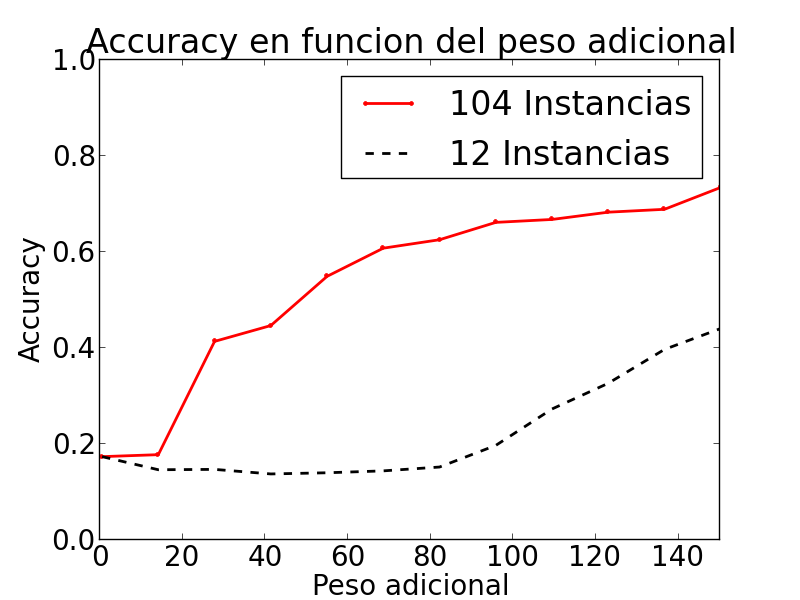
\includegraphics[width=7cm]{accuracy-vs-feat-boost-2corpus}
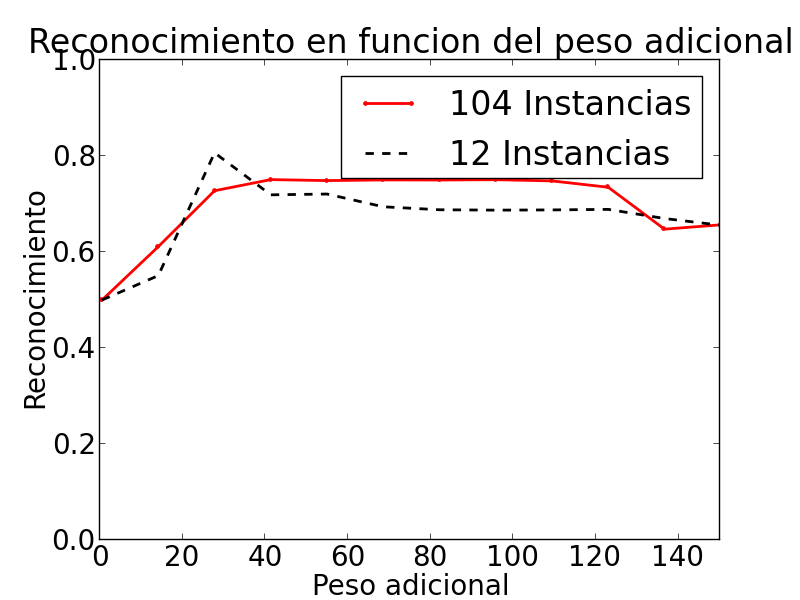
\includegraphics[width=7cm]{recog-vs-feat-boost-2corpus}
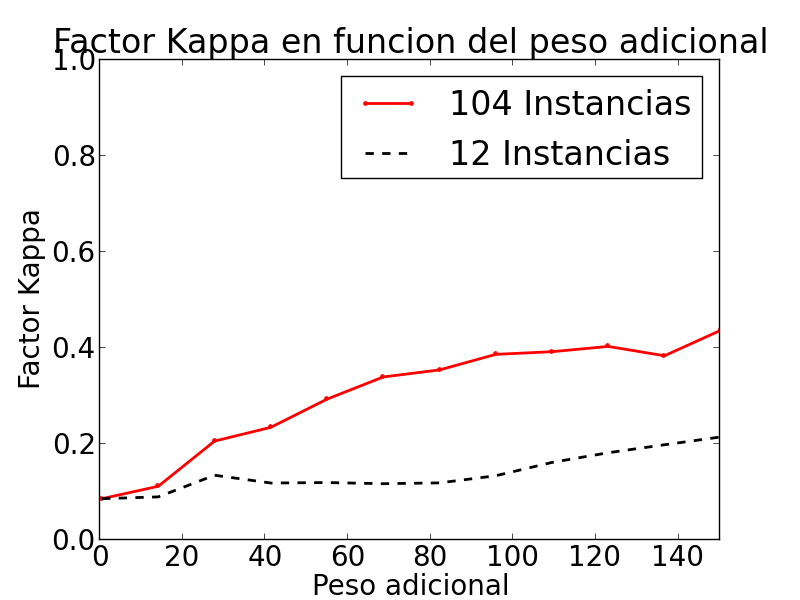
\includegraphics[width=7cm]{kappa-vs-feat-boost-2corpus}
\caption{Rendimiento del clasificador entrenado con características para distintos pesos adicionales entrenado con dos corpus distintos.}
\end{figure}

En la figura \ref{comp-feat-tr-inst} se muestra el \textit{accuracy} y reconocimiento para el clasificador entrenado con y sin características, utilizando distintas cantidades de instancias.

\begin{figure}[h!]\label{comp-feat-tr-inst}
\centering
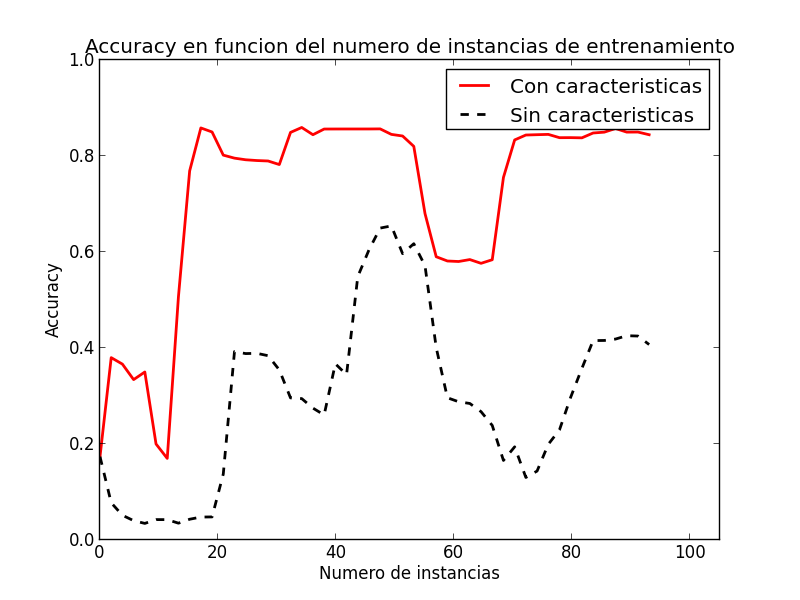
\includegraphics[width=7cm]{accuracy-vs-instancia-feat}
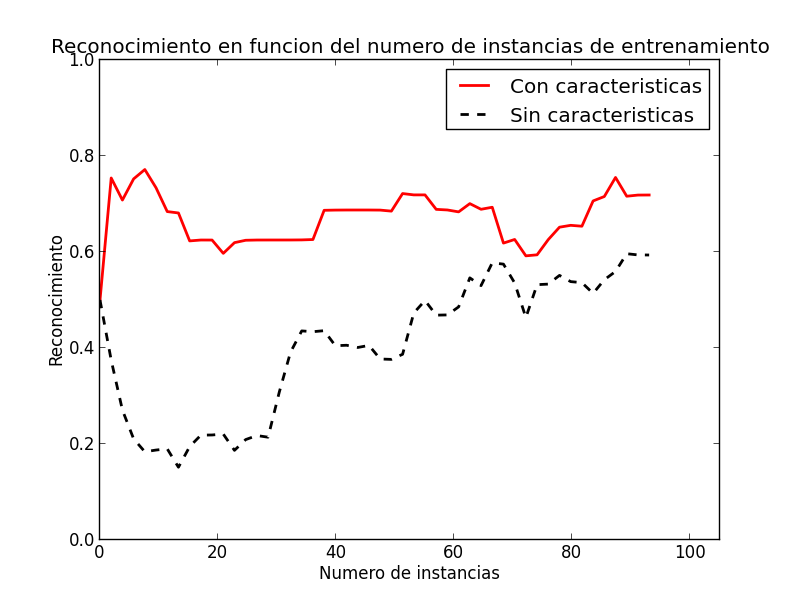
\includegraphics[width=7cm]{recog-vs-instancia-feat}
\caption{Rendimiento del clasificador entrenado con características con un peso adicional de 100 sobre distintas cantidades de instancias.}
\end{figure}
\vspace{3 mm}

\textbf{Conclusión}
Comenzamos por evaluar cuál era el mejor valor posible para el parámetro $\alpha$ y obtuvimos resultados que no se corresponden con los experimentos de \citet{dualist}. Si bien para el reconocimiento el valor del peso adicional no tiene grandes variaciones, el crecimiento es casi proporcional para el \textit{accuracy}. Al no existir etiquetas para la clase \textit{other} introducir pesos en las características crea un límite que le permite al clasificador distinguir las instancias de la clase mayoritaria sin perder reconocimiento. Mientras mayor es el peso adicional, más clara es la línea de separación.

Podemos observar en la imagen \ref{comp-feat-tr-inst} que la separación entre las curvas de aprendizaje entrenando con y sin características se mantiene aproximadamente constante a partir de las 20 instancias. Por otra parte, para el reconocimiento no ocurre lo mismo sino que se cumple nuestra hipótesis de que la contribución del corpus de características disminuiría al agregar instancias. Esto se debe principalmente a que no hay etiquetas para la clase \textit{other} en el corpus de características.

Notamos también que agregar más de 20 instancias no afecta en gran medida ni el \textit{accuracy} ni el reconocimiento ya que gran parte de la información aportada por estas instancias también está representada en el corpus de características. Sin embargo, nosotros hemos etiquetado la mayoría de las características extraídas del estas instancias que estamos agregando. En una sesión de aprendizaje activo real el usuario etiquetaría instancias que probablemente tengan características que no sean redundantes y entonces se justificaría el entrenamiento con gran número de instancias y características.

Utilizar pesos adicionales con valores tan altos no es intuitivo y parece extremo, ya que no se espera que una característica sea 100 o 150 veces más representativa de una clase que otra. Sin embargo, obtenemos estos resultados extremos ya que el corpus con el que estamos trabajando es muy pequeño y la información que de otra forma estaría presente en las instancias de entrenamiento se encuentra directamente en las características. Por ello, para el corpus con menos instancias es necesario pesos adicionales más grandes para aumentar el accuracy.

\section{Experimento 7}
\vspace{3 mm}
\textbf{Hipótesis} El aprendizaje activo sobre características permite al clasificador aprender más rápidamente.
\vspace{3 mm}

Al igual que en el experimento \ref{experimento-aa-instancias}, compararemos estrategias inteligentes de selección de características para agregar al corpus contra la selección aleatoria. Como propusimos en la sección \ref{instance-selection} utilizaremos la ganancia de información de cada característica como estrategia de selección.

La ganancia de información está intímamente relacionada con la entropía. Con las mismas hipótesis del experimento \ref{experimento-aa-instancias} creemos que seleccionar en una primera instancia características que tengan una menor ganancia de información permitirá al clasificador evitar errores que surjan de un entrenamiento con tan pocos ejemplos. Realizaremos entonces experimentos asignando mayor relevancia a mayor ganancia de información y viceversa.

Utilizaremos el clasificador \textit{FeatMultinomialNB} con un peso adicional de 100 para las características etiquetadas. Como no estamos interactuando con un usuario, no necesitamos decidir primero sobre que clase etiquetaremos caracteristicas sino simplemente agregaremos al conjunto de entrenamiento la característica seleccionada por la estrategia con todas las clases con las que esté asociada.

Inicialmente vamos a utilizar el clasificador entrenado con todas las instancias anotadas para medir el impacto de las caracerísticas correctamente.

\vspace{3 mm}

\textbf{Resultados} En la figura \ref{comp-feat-selection} se muestran las curvas de aprendizaje y reconocimiento del clasificador en función de la cantidad de características del corpus utilizadas en el entrenamiento y con distintas estrategias de selección de características. Al graficar las curvas con selección aleatoria tomamos un promedio de 5 ejecuciones del mismo experimento.

\begin{figure}[h!]\label{comp-feat-selection}
\centering
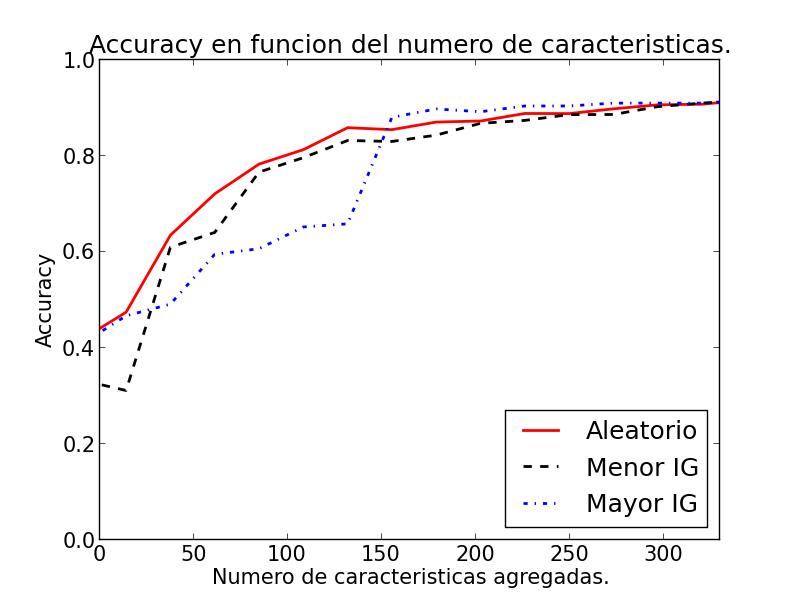
\includegraphics[width=9cm]{learningcurve-aa-feat}
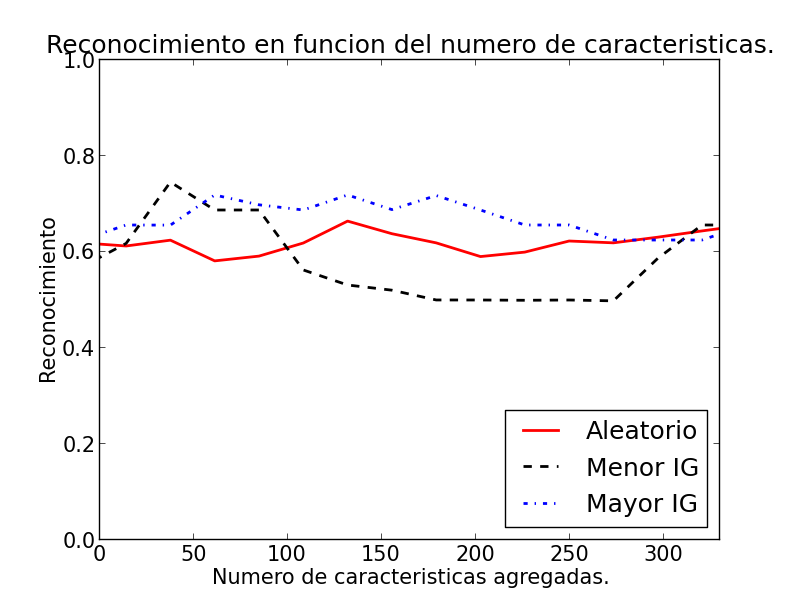
\includegraphics[width=9cm]{recognitioncurve-aa-feat}
\caption{Curvas de aprendizaje y reconocimiento del clasificador entrenado con características con un peso adicional de 100.}
\end{figure}
\vspace{3 mm}


\textbf{Conclusión}
Una vez más hemos conseguido resultados similares utilizando estrategias con alta o baja ganancia de información. Podemos observar en la figura \ref{comp-feat-selection} que hasta la incorporación de 100 instancias la estrategia con menor ganancia de información hace que las curvan crezcan rápidamente, pero a partir de ese punto la mejor forma de selección es utilizando máxima ganancia de información. Es lógico pensar entonces en que combinar estas dos estrategias logrará el máximo rendimiento del clasificador.

%Sin embargo, las dos estrategias superan por poco margen a la selección aleatoria. En estos experimentos se están seleccionando las etiquetas para ser agregadas al corpus de características, lo que no ocurre en una
La cantidad de características agregadas afecta muy poco al reconocimiento final mientras que duplica el \textit{accuracy}.  POR QUE????

El aprendizaje activo sobre características es una buena opción si conseguir instancias es muy dificultoso, ya que en cualquier conjunto de preguntas aleatorio el usuario estaría todo el tiempo etiquetando instancias que no son relevantes.


% \subsection{Hipótesis 2}
% \textbf{El aprendizaje activo sobre instancias y características obtiene mejores resultados que el aprendizaje activo sobre instancias o características por separado.}

% \subsection{Experimento 4}
% \textbf{Hipótesis} ??.

% \subsection{Experimento 5}
% \textbf{Hipótesis} Seleccionar features para etiquetar que tengan alta confiabilidad/correlación, y luego de superado un cierto límite pasar a los que tiene baja confiabilidad/correlación permite al clasificador eliminar el ruido no introducido por la baja cantidad de ejemplos y al mismo tiempo expandir la cobertura.
% Dejar para mas adelante

% Experimento 6
% Information gain sobre todo el corpus o solo el etiquetado.
% IG sobre el corpus anotado + frecuencia en no anotado vs IG sobre todo el corpus anotado y no anotado.

% Experimento 7
% Coocurrencia de features con otros features. (Información mutua)
% Un feature se rankea mas alto si coocurre con features que se rankean alto. Tomando como base la frecuencia.

% Experimento 8
% Information gain sirve o alcanza sólo con usar coocurrencia? Para esto podemos ver la posicion de los features que elige el usuario.
